\documentclass{beamer}
\usepackage{../../shared/styles/custom}
\usepackage{../../shared/styles/conventions}

\def\checkmark{\tikz\fill[scale=0.4](0,.35) -- (.25,0) -- (1,.7) -- (.25,.15) -- cycle;}

%\beamerdefaultoverlayspecification{<+->}

\title{Ridge Regression}
\date{\today}
\author{Nipun Batra}
\institute{IIT Gandhinagar}
\begin{document}
  \maketitle

\begin{frame}{Outline}
\tableofcontents
\end{frame}

\section{Motivation: The Problem of Overfitting}

\begin{frame}{The Problem: Overfitting in Linear Regression}
\begin{alertbox}{Overfitting Challenge}
As model complexity increases (higher polynomial degree), we often observe:
\begin{itemize}
\item Training error decreases
\item Test error increases  
\item Model coefficients become very large
\end{itemize}
\end{alertbox}
\pause

\begin{keypointsbox}{Key Insight}
Large coefficient magnitudes often indicate overfitting!
\end{keypointsbox}
\pause

In polynomial $f(x) = c_0 + c_1x + c_2x^2 + \dots + c_dx^d$, watch $\max|c_i|$
\end{frame}
  
\begin{frame}{Demonstration: Polynomial Degree vs Overfitting}
\vspace{0.4cm}
\only<1>{\begin{figure}\includegraphics[width=0.8\linewidth]{../assets/ridge-regression/figures/lin_1.pdf}\caption{Base Data Set}
\end{figure}}
\only<2>{\begin{figure}\includegraphics[width=0.8\linewidth]{../assets/ridge-regression/figures/lin_plot_1.pdf}\caption{Fit with Degree 1 - Underfitting}
\end{figure}}
\only<3>{\begin{figure}\includegraphics[width=0.8\linewidth]{../assets/ridge-regression/figures/lin_plot_3.pdf}\caption{Fit with Degree 3 - Good Fit}
\end{figure}}
\only<4>{\begin{figure}\includegraphics[width=0.8\linewidth]{../assets/ridge-regression/figures/lin_plot_6.pdf}\caption{Fit with Degree 6 - Starting to Overfit}
\end{figure}}
\only<5>{\begin{figure}\includegraphics[width=0.8\linewidth]{../assets/ridge-regression/figures/lin_plot_11.pdf}\caption{Fit with Degree 11 - Severe Overfitting}
\end{figure}}
\end{frame}  

\begin{frame}{Coefficient Explosion with Overfitting}
\begin{keypointsbox}{Key Observation}
As polynomial degree increases $\rightarrow$ coefficients grow exponentially!
\end{keypointsbox}
\vspace{0.05cm}
\begin{figure}\includegraphics[width=0.65\linewidth]{../assets/ridge-regression/figures/lin_plot_coef.pdf}\caption{{\footnotesize Coefficient Magnitudes vs Polynomial Degree}}\end{figure}
\end{frame}

\begin{frame}{The Central Question}
\begin{alertbox}{Critical Question}
How can we control coefficient magnitudes to prevent overfitting?
\end{alertbox}
\pause

\begin{keypointsbox}{Answer Preview}
Ridge regression adds a penalty term to shrink coefficients!
\end{keypointsbox}
\end{frame}

\stepcounter{popquiz}
\begin{frame}{Pop Quiz \thepopquiz}
\begin{popquizbox}{Pop Quiz \thepopquiz}
Which statement about overfitting is TRUE?
\begin{enumerate}[A)]
\item Higher polynomial degree always improves generalization
\item Large coefficients indicate good model fit
\item Overfitting occurs when training error $>>$ test error
\item Overfitting occurs when training error $<<$ test error
\end{enumerate}
\end{popquizbox}
\end{frame}

\begin{frame}{Answer: Pop Quiz \thepopquiz}
\begin{popquizbox}{Answer: Pop Quiz \thepopquiz}
\textbf{D) Overfitting occurs when training error $<<$ test error}

\vspace{0.3cm}
Explanation:
\begin{itemize}
\item Training error becomes very small (model memorizes training data)
\item Test error remains large (model fails to generalize)  
\item Large gap indicates overfitting
\end{itemize}
\end{popquizbox}
\end{frame}

\section{Ridge Regression Formulation}

\begin{frame}{Solution: Regularization}
\begin{theorembox}{Ridge Regression Approach}
Add a penalty term to control coefficient magnitudes:
\end{theorembox}
\pause

\begin{definitionbox}{Constrained Formulation}
\begin{align*}
\min_{\vtheta} & \quad \left(\vy-\mX\vtheta\right)^T\left(\vy-\mX\vtheta\right) \\
\text{subject to} & \quad \vtheta^T\vtheta \leq S
\end{align*}
where $S > 0$ controls the size of the coefficient vector.
\end{definitionbox}
\end{frame}

\begin{frame}{Lagrangian Formulation}
\begin{theorembox}{Equivalence Theorem}
The constrained problem is equivalent to the unconstrained:
$$\min_{\vtheta} \quad \left(\vy-\mX\vtheta\right)^T\left(\vy-\mX\vtheta\right) + \lambda \vtheta^T\vtheta$$
where $\lambda \geq 0$ is the regularization parameter.
\end{theorembox}
\pause

\begin{keypointsbox}{Key Insight}
This transforms a constrained optimization into an unconstrained one with a penalty term.
\end{keypointsbox}
\end{frame}

\begin{frame}{Understanding the Ridge Penalty}
\begin{align}
J(\vtheta) &= \underbrace{\left(\vy-\mX\vtheta\right)^T\left(\vy-\mX\vtheta\right)}_{\text{Fit to data (MSE)}} + \underbrace{\lambda \vtheta^T\vtheta}_{\text{Penalty term}} \\[0.5em]
&= \text{MSE}(\vtheta) + \lambda \|\vtheta\|_2^2
\end{align}
\pause

\begin{keypointsbox}{Key Components}
\begin{itemize}
\item \textbf{Data fitting term}: Ensures good fit to training data
\item \textbf{Regularization term}: $L_2$ penalty shrinks coefficients toward zero
\item \textbf{$\lambda$}: Controls trade-off between fitting vs. regularization
\end{itemize}
\end{keypointsbox}
\end{frame}

\begin{frame}{Effect of Regularization Parameter $\lambda$}
\begin{keypointsbox}{Parameter Effects}
\begin{itemize}
\item $\lambda = 0$: No regularization (standard linear regression)
\item $\lambda$ small: Light regularization (slight shrinkage)
\item $\lambda$ large: Heavy regularization (strong shrinkage)
\item $\lambda \to \infty$: Extreme regularization (coefficients $\to 0$)
\end{itemize}
\end{keypointsbox}
\pause

\begin{alertbox}{Key Trade-off}
Higher $\lambda$ = more regularization = more bias, less variance
\end{alertbox}
\end{frame}

\begin{frame}{Geometric Interpretation}
\begin{figure}
\centering
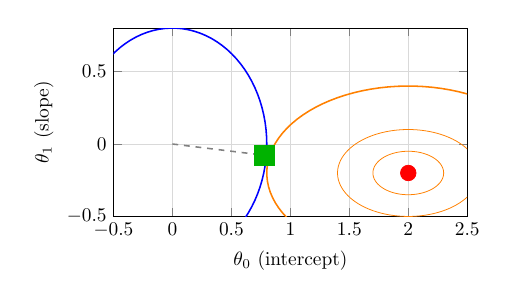
\begin{tikzpicture}[scale=0.7]
\begin{axis}[
    width=8cm, height=5cm,
    xlabel={$\theta_0$ (intercept)}, ylabel={$\theta_1$ (slope)},
    xmin=-0.5, xmax=2.5, ymin=-0.5, ymax=0.8,
    grid=major, grid style={thin,gray!30},
    legend to name=legend3,
    axis equal=false
]
% Constraint circle for Ridge (centered at origin)
\addplot[blue, thick, domain=0:360, samples=100] ({0.8*cos(x)}, {0.8*sin(x)});
% OLS solution point
\addplot[only marks, mark=*, mark size=4pt, red] coordinates {(2.0, -0.2)};
% MSE contour ellipses (centered around OLS)
\addplot[orange, domain=0:360, samples=100] ({0.3*cos(x) + 2.0}, {0.15*sin(x) - 0.2});
\addplot[orange, domain=0:360, samples=100] ({0.6*cos(x) + 2.0}, {0.3*sin(x) - 0.2});
% Critical MSE contour that is tangent to constraint circle
\addplot[orange, thick, domain=0:360, samples=100] ({1.2*cos(x) + 2.0}, {0.6*sin(x) - 0.2});
% Ridge solution point at actual tangency point (where line from OLS to origin intersects constraint circle)
% The tangency occurs along the line from OLS (2.0, -0.2) toward origin
% Direction vector: (-2.0, 0.2), normalized and scaled to radius 0.8
\addplot[only marks, mark=square*, mark size=5pt, green!70!black] coordinates {(0.781, -0.078)};
% Add line showing the tangent direction
\draw[dashed, gray, thick] (axis cs:0,0) -- (axis cs:0.781,-0.078);
% Add invisible point for legend
\addplot[only marks, mark=square*, mark size=0pt, green!70!black] coordinates {(0,0)};
\legend{Constraint $\|\vtheta\|^2 \leq S$, OLS, MSE contours, Ridge Solution}
\end{axis}
\end{tikzpicture}
\vspace{-0.2cm}
\ref{legend3}
\caption{{\small Ridge solution where MSE contours touch constraint region}}
\end{figure}

\vspace{-0.2cm}
\begin{keypointsbox}{Key Insight}
{\small Ridge finds the minimum MSE point within the constraint $\|\vtheta\|_2^2 \leq S$}
\end{keypointsbox}
\end{frame}

\section{Mathematical Derivation}

\begin{frame}{Mathematical Derivation: Step 1}
\begin{codebox}{Step 1: Set up the Lagrangian}
{\small For the constrained optimization problem:}
\begin{align*}
\min_{\vtheta} & \quad \left(\vy-\mX\vtheta\right)^T\left(\vy-\mX\vtheta\right) \\
\text{s.t.} & \quad \vtheta^T\vtheta \leq S
\end{align*}

{\small The Lagrangian is:}
$$L(\vtheta, \lambda) = \left(\vy-\mX\vtheta\right)^T\left(\vy-\mX\vtheta\right) + \lambda\left(\vtheta^T\vtheta - S\right)$$
{\small where $\lambda \geq 0$ is the Lagrange multiplier.}
\end{codebox}
\end{frame}

\begin{frame}{Mathematical Derivation: Step 2}
\begin{codebox}{Step 2: Apply KKT Conditions}
For optimality, we need:
\begin{align}
\frac{\partial L}{\partial \vtheta} &= 0 \quad \text{(stationarity)} \\
\lambda &\geq 0 \quad \text{(dual feasibility)} \\
\vtheta^T\vtheta - S &\leq 0 \quad \text{(primal feasibility)} \\
\lambda(\vtheta^T\vtheta - S) &= 0 \quad \text{(complementary slackness)}
\end{align}
\end{codebox}
\pause

\begin{keypointsbox}{Two Cases}
\begin{itemize}
\item \textbf{Case 1:} $\lambda = 0 \Rightarrow$ No constraint active (standard OLS)
\item \textbf{Case 2:} $\lambda > 0 \Rightarrow$ $\vtheta^T\vtheta = S$ (constraint is tight)
\end{itemize}
\end{keypointsbox}
\end{frame}

\begin{frame}{Mathematical Derivation: Step 3}
\begin{codebox}{Step 3: Compute the Gradient}
Taking the derivative of the Lagrangian with respect to $\vtheta$:
{\small
\begin{align}
\frac{\partial L}{\partial \vtheta} &= \frac{\partial}{\partial \vtheta}\left[\left(\vy-\mX\vtheta\right)^T\left(\vy-\mX\vtheta\right) + \lambda \vtheta^T\vtheta\right] \\[0.2em]
&= \frac{\partial}{\partial \vtheta}\left[\vy^T\vy - 2\vy^T\mX\vtheta + \vtheta^T\mX^T\mX\vtheta + \lambda \vtheta^T\vtheta\right] \\[0.2em]
&= -2\mX^T\vy + 2\mX^T\mX\vtheta + 2\lambda\vtheta
\end{align}
}
\end{codebox}
\end{frame}

\begin{frame}{Mathematical Derivation: Step 4}
\begin{codebox}{Step 4: Set Gradient to Zero}
Setting $\frac{\partial L}{\partial \vtheta} = 0$:
\begin{align}
-2\mX^T\vy + 2\mX^T\mX\vtheta + 2\lambda\vtheta &= 0 \\[0.3em]
-\mX^T\vy + (\mX^T\mX + \lambda\mI)\vtheta &= 0 \\[0.3em]
(\mX^T\mX + \lambda\mI)\vtheta &= \mX^T\vy
\end{align}
\end{codebox}
\pause

\begin{theorembox}{Ridge Regression Solution}
$$\hat{\vtheta}_{\text{ridge}} = (\mX^T\mX + \lambda\mI)^{-1}\mX^T\vy$$
\end{theorembox}

Compare with OLS: $\hat{\vtheta}_{\text{OLS}} = (\mX^T\mX)^{-1}\mX^T\vy$
\end{frame}

\begin{frame}{Effect of Regularization Parameter $\lambda$}
\vspace{0.4cm}
\only<1>{\begin{figure}\includegraphics[width=0.8\linewidth]{../assets/ridge-regression/figures/ridge_1.pdf}\caption{$\lambda = 1$ - Mild Regularization}
\end{figure}}
\only<2>{\begin{figure}\includegraphics[width=0.8\linewidth]{../assets/ridge-regression/figures/ridge_10.pdf}\caption{$\lambda = 10$ - Moderate Regularization}
\end{figure}}
\only<3>{\begin{figure}\includegraphics[width=0.8\linewidth]{../assets/ridge-regression/figures/ridge_1000.pdf}\caption{$\lambda = 1000$ - Heavy Regularization}
\end{figure}}
\end{frame}

%\begin{frame}{Effect of $\mu$ on higher degree fits}
%\vspace{0.4cm}
%\only<1>{\begin{figure}\includegraphics[width=0.8\linewidth]{ridge/ridge_1_16.pdf}\caption{$\mu = 1$ when Degree $= 16$}
%\end{figure}}
%\only<2>{\begin{figure}\includegraphics[width=0.8\linewidth]{ridge/ridge_100_16.pdf}\caption{$\mu = 100$  when Degree $= 16$}
%\end{figure}}
%\only<3>{\begin{figure}\includegraphics[width=0.8\linewidth]{ridge/ridge_100000_16.pdf}\caption{$\mu = 100000$  when Degree $= 16$}
%\end{figure}}
%\end{frame}

\stepcounter{popquiz}
\begin{frame}{Pop Quiz \thepopquiz}
\begin{popquizbox}{Pop Quiz \thepopquiz}
What happens to the Ridge regression solution as $\lambda \to \infty$?
\begin{enumerate}[A)]
\item Coefficients approach the OLS solution
\item Coefficients approach zero
\item Solution becomes undefined
\item Training error becomes zero
\end{enumerate}
\end{popquizbox}
\end{frame}

\begin{frame}{Answer: Pop Quiz \thepopquiz}
\begin{popquizbox}{Answer: Pop Quiz \thepopquiz}
\textbf{B) Coefficients approach zero}

\vspace{0.3cm}
As $\lambda \to \infty$, the penalty term dominates:
$$\hat{\vtheta}_{\text{ridge}} = (\mX^T\mX + \lambda\mI)^{-1}\mX^T\vy \approx \lambda^{-1}\mI \mX^T\vy \to \mathbf{0}$$
\end{popquizbox}
\end{frame}

\begin{frame}{Coefficient Shrinkage: Visual Evidence}
\begin{figure}\includegraphics[width=0.75\linewidth]{../assets/ridge-regression/figures/rid_reg-without-lim.pdf}\caption{{\footnotesize Coefficient Magnitudes vs $\lambda$ (Real Estate Dataset)}}
\end{figure}

\begin{alertbox}{Important Question}
Do coefficients ever become exactly zero?
\end{alertbox}
\end{frame}

\begin{frame}{Ridge Coefficient Behavior}
\begin{figure}\includegraphics[width=0.8\linewidth]{../assets/ridge-regression/figures/rid_reg-with-lim.pdf}\caption{Ridge Coefficients Shrink but Never Reach Zero}
\end{figure}
\end{frame}

\begin{frame}{Ridge vs. Lasso: Key Difference}
\begin{keypointsbox}{Coefficient Behavior Comparison}
\begin{itemize}
\item \textbf{Ridge ($L_2$):} Coefficients shrink toward zero but remain non-zero
\item \textbf{Lasso ($L_1$):} Coefficients can become exactly zero (feature selection)
\end{itemize}
\end{keypointsbox}
\pause

\begin{alertbox}{Important Insight}
Ridge provides shrinkage, Lasso provides selection!
\end{alertbox}
\end{frame}

\begin{frame}{Ridge Regression Solution}
\begin{theorembox}{Ridge Solution Formula}
$$\hat{\vtheta}_{\text{ridge}} = (\mX^T\mX + \lambda\mI)^{-1}\mX^T\vy$$
\end{theorembox}
\end{frame}

\begin{frame}{Key Property 1: Always Invertible}
\begin{theorembox}{Invertibility Guarantee}
$(\mX^T\mX + \lambda\mI)$ is always positive definite for $\lambda > 0$
\end{theorembox}
\pause

\begin{keypointsbox}{Why This Matters}
\begin{itemize}
\item No singularity issues (unlike OLS)
\item Always has unique solution
\item Handles multi-collinearity gracefully
\end{itemize}
\end{keypointsbox}
\end{frame}

\begin{frame}{Key Property 2: Coefficient Shrinkage}
\begin{theorembox}{Shrinkage Effect}
Ridge regression shrinks coefficients toward zero (but not exactly zero)
\end{theorembox}
\pause

\begin{keypointsbox}{Shrinkage Benefits}
\begin{itemize}
\item Reduces overfitting
\item Stabilizes coefficient estimates
\item Improves generalization
\end{itemize}
\end{keypointsbox}
\end{frame}

\begin{frame}{Key Property 3: Bias-Variance Trade-off}
\begin{theorembox}{Trade-off Effect}
Ridge regression increases bias but reduces variance
\end{theorembox}
\pause

\begin{keypointsbox}{Net Effect}
\begin{itemize}
\item Total error often decreases
\item Better generalization to new data
\item Controlled by $\lambda$ parameter
\end{itemize}
\end{keypointsbox}
\end{frame}

\section{Hyperparameter Selection}

\begin{frame}{Choosing the Regularization Parameter $\lambda$}
\begin{alertbox}{Hyperparameter Selection}
How do we choose the optimal value of $\lambda$?
\end{alertbox}
\pause

\begin{theorembox}{Cross-Validation Approach}
\begin{enumerate}
\item Split data into training and validation sets (k-fold CV)
\item For each candidate $\lambda$ value:
   \begin{itemize}
   \item Train ridge model on training data
   \item Compute validation error
   \end{itemize}
\item Select $\lambda$ that minimizes validation error
\item Retrain on full dataset with chosen $\lambda$
\end{enumerate}
\end{theorembox}
\end{frame}

\begin{frame}{Cross-Validation for Ridge Regression}
\begin{figure}
\centering
\includegraphics[width=0.75\linewidth]{ridge-cv.pdf}
\caption{{\small Cross-validation curve showing optimal $\lambda$}}
\end{figure}

\vspace{-0.1cm}
\begin{keypointsbox}{CV Pattern}
{\footnotesize 
Small $\lambda$: Overfitting \quad Large $\lambda$: Underfitting \quad Optimal $\lambda$: Best trade-off
}
\end{keypointsbox}
\end{frame}

\begin{frame}{Bias-Variance Trade-off in Ridge Regression}
\begin{theorembox}{Bias-Variance Decomposition}
Total Error = Bias$^2$ + Variance + Irreducible Error
\end{theorembox}
\pause

\begin{keypointsbox}{Ridge Effect}
Regularization increases bias but reduces variance, often leading to lower total error.
\end{keypointsbox}
\end{frame}

\begin{frame}{Small vs Large Regularization}
\begin{columns}
\begin{column}{0.48\textwidth}
\begin{figure}
\includegraphics[width=\linewidth]{../assets/ridge-regression/figures/ridge_new_0_17.pdf}
\end{figure}
\textbf{Small $\lambda$ ($\lambda \to 0$):}
\begin{itemize}
\item Low bias
\item High variance
\item Risk of overfitting
\end{itemize}
\end{column}
\begin{column}{0.48\textwidth}
\begin{figure}
\includegraphics[width=\linewidth]{../assets/ridge-regression/figures/ridge_new_1_17.pdf}
\end{figure}
\textbf{Large $\lambda$ ($\lambda \to \infty$):}
\begin{itemize}
\item High bias
\item Low variance  
\item Risk of underfitting
\end{itemize}
\end{column}
\end{columns}
\end{frame}

\stepcounter{popquiz}
\begin{frame}{Pop Quiz \thepopquiz}
\begin{popquizbox}{Pop Quiz \thepopquiz}
In ridge regression, as we increase $\lambda$, what happens to model bias and variance?
\begin{enumerate}[A)]
\item Both bias and variance increase
\item Both bias and variance decrease
\item Bias increases, variance decreases
\item Bias decreases, variance increases
\end{enumerate}
\end{popquizbox}
\end{frame}

\begin{frame}{Answer: Pop Quiz \thepopquiz}
\begin{popquizbox}{Answer: Pop Quiz \thepopquiz}
\textbf{C) Bias increases, variance decreases}

\vspace{0.3cm}
Explanation:
\begin{itemize}
\item Increasing $\lambda$ constrains coefficients more severely
\item Model becomes simpler (higher bias)
\item Less sensitive to training data variations (lower variance)
\item This is the fundamental bias-variance trade-off!
\end{itemize}
\end{popquizbox}
\end{frame}

\section{Examples and Applications}

\begin{frame}{Worked Example: Setup}
\begin{examplebox}{Ridge Regression Example}
Given the following simple dataset, compare OLS vs. Ridge regression with $\lambda = 2$:

\vspace{0.3cm}
Data: $(x_1, y_1) = (1, 1)$, $(x_2, y_2) = (2, 2)$, $(x_3, y_3) = (3, 3)$, $(x_4, y_4) = (4, 0)$

Model: $y = \theta_0 + \theta_1 x$
\end{examplebox}
\pause

\begin{codebox}{Step 1: Set up matrices}
$$\mX = \begin{bmatrix} 1 & 1 \\ 1 & 2 \\ 1 & 3 \\ 1 & 4 \end{bmatrix}, \quad \vy = \begin{bmatrix} 1 \\ 2 \\ 3 \\ 0 \end{bmatrix}, \quad \vtheta = \begin{bmatrix} \theta_0 \\ \theta_1 \end{bmatrix}$$
\end{codebox}
\end{frame}

\begin{frame}{Worked Example: OLS Setup}
\begin{codebox}{Step 2: Ordinary Least Squares}
$$\hat{\vtheta}_{\text{OLS}} = (\mX^{T}\mX)^{-1}(\mX^{T}\vy)$$
\end{codebox}
\pause

\begin{codebox}{Step 3: Compute matrix products}
\begin{align*}
\mX^{T}\mX &= \begin{bmatrix} 4 & 10 \\ 10 & 30 \end{bmatrix} \\
\mX^{T}\vy &= \begin{bmatrix} 6 \\ 14 \end{bmatrix}
\end{align*}
\end{codebox}
\end{frame}

\begin{frame}{Worked Example: Matrix Inverse}
\begin{codebox}{Step 4: Compute the inverse}
For $\mX^T\mX = \begin{bmatrix} 4 & 10 \\ 10 & 30 \end{bmatrix}$:

$\det(\mX^T\mX) = 4 \cdot 30 - 10 \cdot 10 = 20$

$$(\mX^{T}\mX)^{-1} = \frac{1}{20} \begin{bmatrix} 30 & -10 \\ -10 & 4 \end{bmatrix}$$
\end{codebox}
\end{frame}

\begin{frame}{Worked Example: OLS Calculation}
\begin{codebox}{Step 5: Final matrix multiplication}
\begin{align*}
\hat{\vtheta}_{\text{OLS}} &= (\mX^{T}\mX)^{-1}(\mX^{T}\vy) \\
&= \frac{1}{20} \begin{bmatrix} 30 & -10 \\ -10 & 4 \end{bmatrix} \begin{bmatrix} 6 \\ 14 \end{bmatrix} \\
&= \frac{1}{20} \begin{bmatrix} 180-140 \\ -60+56 \end{bmatrix} = \frac{1}{20} \begin{bmatrix} 40 \\ -4 \end{bmatrix} = \begin{bmatrix} 2.0 \\ -0.2 \end{bmatrix}
\end{align*}
\end{codebox}
\end{frame}

\begin{frame}{OLS Final Result}
\begin{theorembox}{OLS Result}
$\hat{y} = 2.0 - 0.2x$ \quad (No regularization)
\end{theorembox}

\begin{figure}
\centering
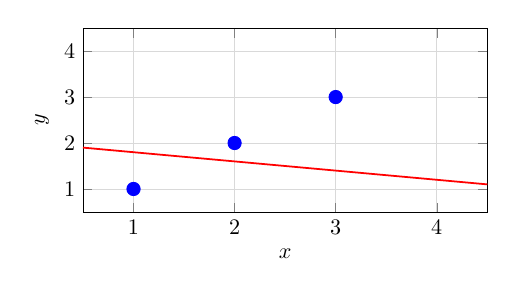
\begin{tikzpicture}[scale=0.8]
\begin{axis}[
    width=8cm, height=4.5cm,
    xlabel={$x$}, ylabel={$y$},
    xmin=0.5, xmax=4.5, ymin=0.5, ymax=4.5,
    grid=major, grid style={thin,gray!30},
    legend to name=legend1
]
% Data points
\addplot[only marks, mark=*, mark size=3pt, blue] coordinates {
    (1,1) (2,2) (3,3) (4,0)
};
% OLS line: y = 2.0 - 0.2x
\addplot[red, thick, domain=0.5:4.5] {2.0 - 0.2*x};
\legend{Data, OLS: $\hat{y} = 2.0 - 0.2x$}
\end{axis}
\end{tikzpicture}
\vspace{-0.2cm}
\ref{legend1}
\caption{{\small OLS fit to our example data}}
\end{figure}
\end{frame}

\begin{frame}{Worked Example: Ridge Setup}
\begin{codebox}{Step 5: Ridge regression with $\lambda = 2$}
$$\hat{\vtheta}_{\text{ridge}} = (\mX^{T}\mX + \lambda\mI)^{-1}(\mX^{T}\vy)$$
\end{codebox}
\pause

\begin{codebox}{Step 6: Add regularization term}
\begin{align*}
\mX^{T}\mX + \lambda\mI &= \begin{bmatrix} 4 & 10 \\ 10 & 30 \end{bmatrix} + 2\mI \\
&= \begin{bmatrix} 6 & 10 \\ 10 & 32 \end{bmatrix}
\end{align*}
\end{codebox}
\end{frame}

\begin{frame}{Worked Example: Matrix Inverse}
\begin{codebox}{Step 7: Compute inverse}
$\det(\mX^T\mX + \lambda\mI) = 6 \cdot 32 - 10 \cdot 10 = 92$

$$(\mX^{T}\mX + \lambda\mI)^{-1} = \frac{1}{92} \begin{bmatrix} 32 & -10 \\ -10 & 6 \end{bmatrix}$$
\end{codebox}
\end{frame}

\begin{frame}{Worked Example: Ridge Calculation}
\begin{codebox}{Step 8: Matrix multiplication}
\begin{align*}
\hat{\vtheta}_{\text{ridge}} &= (\mX^{T}\mX + \lambda\mI)^{-1}(\mX^{T}\vy) \\
&= \frac{1}{92} \begin{bmatrix} 32 & -10 \\ -10 & 6 \end{bmatrix} \begin{bmatrix} 6 \\ 14 \end{bmatrix}
\end{align*}
\end{codebox}
\pause

\begin{codebox}{Step 9: Compute products}
\begin{align*}
&= \frac{1}{92} \begin{bmatrix} 32 \cdot 6 + (-10) \cdot 14 \\ (-10) \cdot 6 + 6 \cdot 14 \end{bmatrix} \\
&= \frac{1}{92} \begin{bmatrix} 192-140 \\ -60+84 \end{bmatrix} = \frac{1}{92} \begin{bmatrix} 52 \\ 24 \end{bmatrix} = \begin{bmatrix} 0.565 \\ 0.261 \end{bmatrix}
\end{align*}
\end{codebox}
\end{frame}

\begin{frame}{Ridge vs OLS: Final Comparison}
\begin{theorembox}{Ridge Result}
$\hat{y} = 0.565 + 0.261x$ \quad (With $\lambda = 2$)
\end{theorembox}

\begin{figure}
\centering
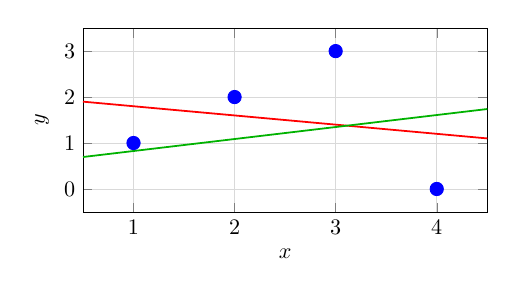
\begin{tikzpicture}[scale=0.8]
\begin{axis}[
    width=8cm, height=4.5cm,
    xlabel={$x$}, ylabel={$y$},
    xmin=0.5, xmax=4.5, ymin=-0.5, ymax=3.5,
    grid=major, grid style={thin,gray!30},
    legend to name=legend2
]
% Data points
\addplot[only marks, mark=*, mark size=3pt, blue] coordinates {
    (1,1) (2,2) (3,3) (4,0)
};
% OLS line: y = 2.0 - 0.2x
\addplot[red, thick, domain=0.5:4.5] {2.0 - 0.2*x};
% Ridge line: y = 0.565 + 0.261x
\addplot[green!70!black, thick, domain=0.5:4.5] {0.565 + 0.261*x};
\legend{Data, OLS: $\hat{y} = 2.0 - 0.2x$, Ridge: $\hat{y} = 0.565 + 0.261x$}
\end{axis}
\end{tikzpicture}
\vspace{-0.3cm}
\ref{legend2}
\caption{{\small Ridge regression provides more stable coefficients}}
\end{figure}
\end{frame}

\begin{frame}{Coefficient Magnitude Comparison}
\begin{theorembox}{OLS vs Ridge Solutions}
\begin{itemize}
\item \textbf{OLS}: $\vtheta_{OLS} = \begin{bmatrix} 2.0 \\ -0.2 \end{bmatrix}$ 
\item \textbf{Ridge}: $\vtheta_{Ridge} = \begin{bmatrix} 0.565 \\ 0.261 \end{bmatrix}$
\end{itemize}
\end{theorembox}
\pause

\begin{codebox}{L2 Norm Calculation}
\begin{align}
\|\vtheta_{OLS}\|_2^2 &= (2.0)^2 + (-0.2)^2 = 4.04 \\
\|\vtheta_{Ridge}\|_2^2 &= (0.565)^2 + (0.261)^2 = 0.387
\end{align}
\end{codebox}
\end{frame}

\begin{frame}{Ridge Coefficient Shrinkage Result}
\begin{alertbox}{Key Result}
Ridge regression achieved a {\bf 90.4\% reduction} in coefficient magnitude!
$$\frac{0.387}{4.04} = 0.096 \quad \text{(Ridge is 9.6\% of OLS magnitude)}$$
\end{alertbox}

\begin{keypointsbox}{Shrinkage Effect}
Ridge systematically produces smaller coefficient magnitudes while maintaining prediction accuracy.
\end{keypointsbox}
\end{frame}

\begin{frame}{Multi-collinearity}
$(\mX^{T}\mX)^{-1}$ is not computable when $|\mX^{T}\mX|$ = 0.

This was a drawback of using linear regression

\begin{equation*}
\mX = \begin{bmatrix}
1 & 1& 2\\
1 & 2& 4\\
1 & 3& 6\\
\end{bmatrix}
\end{equation*}

The matrix $\mX$ is not full rank. 
\end{frame}

\begin{frame}{Ridge Solution to Multi-collinearity}
\begin{keypointsbox}{Ridge Advantage}
With ridge regression, we invert $\mX^{T}\mX + \mu \mI$ instead of $\mX^{T}\mX$
\end{keypointsbox}

\begin{equation*}
\mX^T\mX + \mu \mI = \begin{bmatrix}
3+\mu & 6& 12\\
6 & 14+\mu & 28\\
12 & 28& 56+\mu \\
\end{bmatrix}
\end{equation*}
\end{frame}

\begin{frame}{Why Ridge Fixes Singularity}
\begin{theorembox}{Key Result}
The matrix $\mX^T\mX + \mu \mI$ is always full rank for $\mu > 0$
\end{theorembox}
\pause

\begin{alertbox}{Another Interpretation}
Ridge regression = regularization = fixing singularity issues!
\end{alertbox}
\pause

\begin{keypointsbox}{Summary}
Ridge regression elegantly handles multi-collinearity problems!
\end{keypointsbox}
\end{frame}


\begin{frame}{The Intercept Penalty Problem}
\begin{alertbox}{Critical Issue}
Should we penalize the intercept $\theta_0$ in ridge regression?
\end{alertbox}

\begin{keypointsbox}{Two Approaches}
\begin{itemize}
\item \textbf{Standard Ridge}: $\hat{\vtheta} = (\mX^T\mX + \lambda\mI)^{-1}\mX^T\vy$ (penalizes intercept)
\item \textbf{No-intercept penalty}: $\hat{\vtheta} = (\mX^T\mX + \lambda\mI^*)^{-1}\mX^T\vy$
\end{itemize}
\end{keypointsbox}
\end{frame}

\begin{frame}{Modified Identity Matrix $\mI^*$}
\begin{codebox}{Definition of $\mI^*$}
$$\mI^* = \begin{bmatrix}
    \color{red}0 & 0 & 0 & \dots  & 0 \\
    0 & 1& 0 & \dots  & 0\\
    \vdots & \vdots & \vdots & \ddots & \vdots \\
    0 & 0 & 0 & \dots  & 1
\end{bmatrix}$$
\end{codebox}

\begin{alertbox}{Key Point}
Zero in first position means NO penalty on intercept $\theta_0$
\end{alertbox}
\end{frame}

\begin{frame}{Demonstration: Two Simple Functions}
\begin{examplebox}{Setup}
Compare two functions with different intercepts:
\begin{itemize}
\item \textbf{Function 1}: $f_1(x) = x$ (small intercept)
\item \textbf{Function 2}: $f_2(x) = x + 100$ (large intercept)
\end{itemize}
\end{examplebox}
\end{frame}

\begin{frame}{Data Generation and Test Question}
\begin{codebox}{Data Generation}
For each function, generate data at $x = 1, 2$:
\begin{align}
\text{Function 1:} &\quad (1,1), (2,2) \\
\text{Function 2:} &\quad (1,101), (2,102)
\end{align}
\end{codebox}
\pause

\begin{alertbox}{Test Question}
How well can we predict $y$ at $x = 0$ using ridge regression with $\lambda = 100$?
\end{alertbox}
\end{frame}

\begin{frame}{Function 1: Setup and Data}
\begin{theorembox}{Function 1: $y = x$}
True value at $x=0$: $y = 0$
\end{theorembox}

\begin{codebox}{Data matrices}
$$\mX = \begin{bmatrix} 1 & 1 \\ 1 & 2 \end{bmatrix}, \quad \vy = \begin{bmatrix} 1 \\ 2 \end{bmatrix}$$
\end{codebox}
\end{frame}

\begin{frame}{Function 1: Matrix Computations}
\begin{codebox}{Matrix computations}
\begin{align}
\mX^T\mX &= \begin{bmatrix} 2 & 3 \\ 3 & 5 \end{bmatrix} \\
\mX^T\vy &= \begin{bmatrix} 3 \\ 5 \end{bmatrix}
\end{align}
\end{codebox}
\end{frame}

\begin{frame}{Function 1: Ridge with Standard $\mI$}
\begin{codebox}{Standard Ridge: $\mI$ penalties both $\theta_0$ and $\theta_1$}
$$\mX^T\mX + \lambda\mI = \begin{bmatrix} 2 & 3 \\ 3 & 5 \end{bmatrix} + 100\begin{bmatrix} 1 & 0 \\ 0 & 1 \end{bmatrix} = \begin{bmatrix} 102 & 3 \\ 3 & 105 \end{bmatrix}$$
\end{codebox}
\end{frame}

\begin{frame}{Function 1: Standard Ridge Solution}
\begin{codebox}{Solution}
\begin{align}
\hat{\vtheta} &= \begin{bmatrix} 102 & 3 \\ 3 & 105 \end{bmatrix}^{-1} \begin{bmatrix} 3 \\ 5 \end{bmatrix} \\
&\approx \begin{bmatrix} 0.029 \\ 0.047 \end{bmatrix}
\end{align}
\end{codebox}
\pause

\begin{theorembox}{Prediction at $x=0$}
$\hat{y}(0) = 0.029 + 0.047 \times 0 = 0.029$ \\
{\small Error: $|0.029 - 0| = 0.029$}
\end{theorembox}
\end{frame}

\begin{frame}{Function 1: Ridge with Modified $\mI^*$}
\begin{codebox}{Modified Ridge: $\mI^*$ does NOT penalize $\theta_0$}
$$\mX^T\mX + \lambda\mI^* = \begin{bmatrix} 2 & 3 \\ 3 & 5 \end{bmatrix} + 100\begin{bmatrix} 0 & 0 \\ 0 & 1 \end{bmatrix} = \begin{bmatrix} 2 & 3 \\ 3 & 105 \end{bmatrix}$$
\end{codebox}
\end{frame}

\begin{frame}{Function 1: Modified Ridge Solution}
\begin{codebox}{Solution}
\begin{align}
\hat{\vtheta} &= \begin{bmatrix} 2 & 3 \\ 3 & 105 \end{bmatrix}^{-1} \begin{bmatrix} 3 \\ 5 \end{bmatrix} \\
&\approx \begin{bmatrix} -0.001 \\ 0.048 \end{bmatrix}
\end{align}
\end{codebox}
\pause

\begin{theorembox}{Prediction at $x=0$}
$\hat{y}(0) = -0.001 + 0.048 \times 0 = -0.001$ \\
{\small Error: $|-0.001 - 0| = 0.001$}
\end{theorembox}
\end{frame}

\begin{frame}{Function 2: Setup and Data}
\begin{theorembox}{Function 2: $y = x + 100$}
True value at $x=0$: $y = 100$
\end{theorembox}

\begin{codebox}{Data matrices}
$$\mX = \begin{bmatrix} 1 & 1 \\ 1 & 2 \end{bmatrix}, \quad \vy = \begin{bmatrix} 101 \\ 102 \end{bmatrix}$$
\end{codebox}
\end{frame}

\begin{frame}{Function 2: Matrix Computations}
\begin{codebox}{Matrix computations}
\begin{align}
\mX^T\mX &= \begin{bmatrix} 2 & 3 \\ 3 & 5 \end{bmatrix} \quad \text{(same as Function 1)} \\
\mX^T\vy &= \begin{bmatrix} 203 \\ 305 \end{bmatrix}
\end{align}
\end{codebox}
\end{frame}

\begin{frame}{Function 2: Ridge with Standard $\mI$}
\begin{codebox}{Standard Ridge: penalizes large intercept heavily}
$$\mX^T\mX + \lambda\mI = \begin{bmatrix} 102 & 3 \\ 3 & 105 \end{bmatrix} \quad \text{(same matrix)}$$
\end{codebox}
\end{frame}

\begin{frame}{Function 2: Standard Ridge Solution}
\begin{codebox}{Solution}
\begin{align}
\hat{\vtheta} &= \begin{bmatrix} 102 & 3 \\ 3 & 105 \end{bmatrix}^{-1} \begin{bmatrix} 203 \\ 305 \end{bmatrix} \\
&\approx \begin{bmatrix} 1.98 \\ 2.89 \end{bmatrix}
\end{align}
\end{codebox}
\pause

\begin{theorembox}{Prediction at $x=0$}
$\hat{y}(0) = 1.98 + 2.89 \times 0 = 1.98$ \\
{\color{red}\textbf{Error: $|1.98 - 100| = 98.02$ (TERRIBLE!)}}
\end{theorembox}
\end{frame}

\begin{frame}{Function 2: Ridge with Modified $\mI^*$}
\begin{codebox}{Modified Ridge: does NOT penalize intercept}
$$\mX^T\mX + \lambda\mI^* = \begin{bmatrix} 2 & 3 \\ 3 & 105 \end{bmatrix} \quad \text{(same as Function 1)}$$
\end{codebox}
\end{frame}

\begin{frame}{Function 2: Modified Ridge Solution}
\begin{codebox}{Solution}
\begin{align}
\hat{\vtheta} &= \begin{bmatrix} 2 & 3 \\ 3 & 105 \end{bmatrix}^{-1} \begin{bmatrix} 203 \\ 305 \end{bmatrix} \\
&\approx \begin{bmatrix} 99.91 \\ 1.05 \end{bmatrix}
\end{align}
\end{codebox}
\pause

\begin{theorembox}{Prediction at $x=0$}
$\hat{y}(0) = 99.91 + 1.05 \times 0 = 99.91$ \\
{\color{green}\textbf{Error: $|99.91 - 100| = 0.09$ (EXCELLENT!)}}
\end{theorembox}
\end{frame}

\begin{frame}{Results Summary}
\begin{table}
\centering
\begin{tabular}{|l|c|c|c|}
\hline
\textbf{Function} & \textbf{True $y(0)$} & \textbf{Standard $\mI$} & \textbf{Modified $\mI^*$} \\
\hline
$f_1: y = x$ & 0 & 0.029 & -0.001 \\
Error & & 0.029 & \color{green}0.001 \\
\hline
$f_2: y = x + 100$ & 100 & 1.98 & 99.91 \\
Error & & \color{red}98.02 & \color{green}0.09 \\
\hline
\end{tabular}
\end{table}
\pause

\begin{alertbox}{Key Insight}
Penalizing the intercept creates \textbf{biased predictions} when data has non-zero mean!
\end{alertbox}
\pause

\begin{keypointsbox}{Solution}
Use $\mI^*$ to avoid penalizing the intercept, or normalize data first.
\end{keypointsbox}
\end{frame}

\begin{frame}{Alternative: Data Normalization}
\begin{theorembox}{Normalization Approach}
Center the data to have zero mean, then use standard $\mI$
\end{theorembox}

\begin{codebox}{Function 2 with normalization}
Original: $(1,101), (2,102)$ \\
Mean: $\bar{x} = 1.5, \bar{y} = 101.5$ \\
Centered: $(-0.5, -0.5), (0.5, 0.5)$
\end{codebox}
\end{frame}

\begin{frame}{Benefits of Data Normalization}
\begin{keypointsbox}{Why Normalize?}
\begin{itemize}
\item Can use standard $\mI$ without bias
\item Intercept becomes meaningful (deviation from mean)
\item All features on similar scale
\item More numerically stable
\end{itemize}
\end{keypointsbox}

\begin{alertbox}{Best Practice}
Always normalize data OR use $\mI^*$ for unbiased ridge regression!
\end{alertbox}
\end{frame}

\section{Implementation Details}

\begin{frame}{Ridge Regression via Gradient Descent}
\begin{theorembox}{Gradient Descent Update Rule}
Standard gradient descent step for ridge regression:
$$\vtheta^{(t+1)} = \vtheta^{(t)} - \alpha \nabla J(\vtheta^{(t)})$$
\end{theorembox}
\pause

\begin{codebox}{Ridge Gradient Computation}
\begin{align}
\nabla J(\vtheta) &= \nabla \left[\frac{1}{2}\|\vy-\mX\vtheta\|_2^2 + \frac{\lambda}{2}\|\vtheta\|_2^2\right] \\
&= -\mX^T(\vy-\mX\vtheta) + \lambda\vtheta \\
&= -\mX^T\vy + \mX^T\mX\vtheta + \lambda\vtheta
\end{align}
\end{codebox}
\end{frame}

\begin{frame}{Ridge vs OLS: Gradient Descent Updates}
\begin{theorembox}{Ridge Update (with shrinkage)}
$$\vtheta^{(t+1)} = \vtheta^{(t)} - \alpha(-\mX^T\vy + \mX^T\mX\vtheta^{(t)} + \lambda\vtheta^{(t)})$$
$$= (1 - \alpha\lambda)\vtheta^{(t)} - \alpha(-\mX^T\vy + \mX^T\mX\vtheta^{(t)})$$
\end{theorembox}
\pause

\begin{theorembox}{OLS Update (no shrinkage)}
$$\vtheta^{(t+1)} = \vtheta^{(t)} - \alpha(-\mX^T\vy + \mX^T\mX\vtheta^{(t)})$$
\end{theorembox}
\pause

\begin{keypointsbox}{Key Insight}
The $(1 - \alpha\lambda)$ factor \textbf{shrinks} coefficients at each step!
\end{keypointsbox}
\end{frame}

\begin{frame}{Visual: OLS Gradient Descent Step}
\begin{columns}
\column{0.5\textwidth}
\begin{theorembox}{OLS Update}
$\vtheta^{(t+1)} = \vtheta^{(t)} - \alpha \nabla J(\vtheta^{(t)})$
\end{theorembox}

\column{0.5\textwidth}
\begin{center}
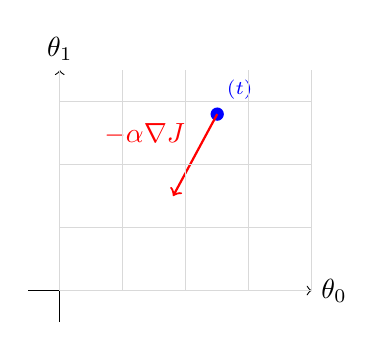
\begin{tikzpicture}[scale=0.8]
  % Axes
  \draw[->] (-0.5,0) -- (4,0) node[right] {$\theta_0$};
  \draw[->] (0,-0.5) -- (0,3.5) node[above] {$\theta_1$};
  
  % Current point theta^(t)
  \coordinate (theta_t) at (2.5, 2.8);
  \fill[blue] (theta_t) circle (3pt);
  \node[blue, above right] at (theta_t) {$\vtheta^{(t)}$};
  
  % Gradient vector -∇J (pointing toward minimum)
  \coordinate (grad_end) at (1.8, 1.5);
  \draw[->, red, thick] (theta_t) -- (grad_end) node[midway, above left] {$-\alpha\nabla J$};
  
  % Grid for reference
  \draw[gray!30, thin] (0,0) grid (4,3.5);
\end{tikzpicture}
\end{center}
\end{columns}

\begin{alertbox}{Step 1}
Start at $\vtheta^{(t)}$ and compute negative gradient direction
\end{alertbox}
\end{frame}

\begin{frame}{Visual: OLS Gradient Descent - Vector Sum}
\begin{columns}
\column{0.5\textwidth}
\begin{theorembox}{Vector Addition}
$\vtheta^{(t+1)} = \vtheta^{(t)} + (-\alpha \nabla J)$
\end{theorembox}

\column{0.5\textwidth}
\begin{center}
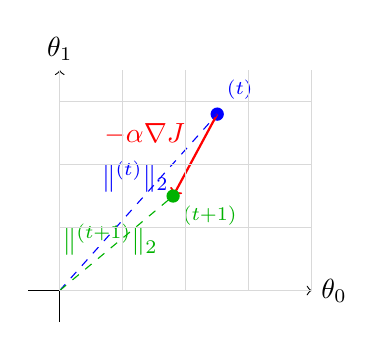
\begin{tikzpicture}[scale=0.8]
  % Axes
  \draw[->] (-0.5,0) -- (4,0) node[right] {$\theta_0$};
  \draw[->] (0,-0.5) -- (0,3.5) node[above] {$\theta_1$};
  
  % Current point theta^(t)
  \coordinate (theta_t) at (2.5, 2.8);
  \fill[blue] (theta_t) circle (3pt);
  \node[blue, above right] at (theta_t) {$\vtheta^{(t)}$};
  
  % Gradient vector
  \coordinate (grad_end) at (1.8, 1.5);
  \draw[->, red, thick] (theta_t) -- (grad_end) node[midway, above left] {$-\alpha\nabla J$};
  
  % New point theta^(t+1)
  \fill[green!70!black] (grad_end) circle (3pt);
  \node[green!70!black, below right] at (grad_end) {$\vtheta^{(t+1)}$};
  
  % Show L2 norm
  \draw[dashed, blue] (0,0) -- (theta_t);
  \draw[dashed, green!70!black] (0,0) -- (grad_end);
  \node[blue] at (1.2, 1.8) {$\|\vtheta^{(t)}\|_2$};
  \node[green!70!black] at (0.8, 0.8) {$\|\vtheta^{(t+1)}\|_2$};
  
  % Grid for reference
  \draw[gray!30, thin] (0,0) grid (4,3.5);
\end{tikzpicture}
\end{center}
\end{columns}

\begin{keypointsbox}{Result}
OLS: $\|\vtheta^{(t+1)}\|_2$ depends only on gradient direction
\end{keypointsbox}
\end{frame}

\begin{frame}{Visual: Ridge Gradient Descent - Shrinkage Step}
\begin{columns}
\column{0.5\textwidth}
\begin{theorembox}{Ridge Shrinkage}
First: $\vtheta^{(t)} \rightarrow (1-\alpha\lambda)\vtheta^{(t)}$
\end{theorembox}

\column{0.5\textwidth}
\begin{center}
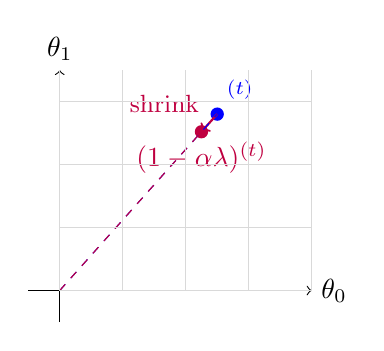
\begin{tikzpicture}[scale=0.8]
  % Axes
  \draw[->] (-0.5,0) -- (4,0) node[right] {$\theta_0$};
  \draw[->] (0,-0.5) -- (0,3.5) node[above] {$\theta_1$};
  
  % Current point theta^(t)
  \coordinate (theta_t) at (2.5, 2.8);
  \fill[blue] (theta_t) circle (3pt);
  \node[blue, above right] at (theta_t) {$\vtheta^{(t)}$};
  
  % Shrunk point
  \coordinate (shrunk) at (2.25, 2.52);
  \fill[purple] (shrunk) circle (3pt);
  \node[purple, below] at (shrunk) {$(1-\alpha\lambda)\vtheta^{(t)}$};
  
  % Shrinkage arrow
  \draw[->, purple, thick] (theta_t) -- (shrunk) node[midway, above left] {\small shrink};
  
  % Show norms
  \draw[dashed, blue] (0,0) -- (theta_t);
  \draw[dashed, purple] (0,0) -- (shrunk);
  
  % Grid for reference
  \draw[gray!30, thin] (0,0) grid (4,3.5);
\end{tikzpicture}
\end{center}
\end{columns}

\begin{alertbox}{Ridge Step 1}
Shrink current parameters by factor $(1-\alpha\lambda) < 1$
\end{alertbox}
\end{frame}

\begin{frame}{Visual: Ridge Gradient Descent - Complete Update}
\begin{columns}
\column{0.5\textwidth}
\begin{theorembox}{Ridge Complete Update}
$\vtheta^{(t+1)} = (1-\alpha\lambda)\vtheta^{(t)} - \alpha\nabla J$
\end{theorembox}

\column{0.5\textwidth}
\begin{center}
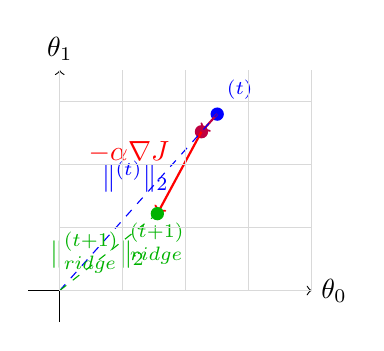
\begin{tikzpicture}[scale=0.8]
  % Axes
  \draw[->] (-0.5,0) -- (4,0) node[right] {$\theta_0$};
  \draw[->] (0,-0.5) -- (0,3.5) node[above] {$\theta_1$};
  
  % Current point theta^(t)
  \coordinate (theta_t) at (2.5, 2.8);
  \fill[blue] (theta_t) circle (3pt);
  \node[blue, above right] at (theta_t) {$\vtheta^{(t)}$};
  
  % Shrunk point
  \coordinate (shrunk) at (2.25, 2.52);
  \fill[purple] (shrunk) circle (3pt);
  \draw[->, purple, thick] (theta_t) -- (shrunk);
  
  % Gradient from shrunk point
  \coordinate (final) at (1.55, 1.22);
  \draw[->, red, thick] (shrunk) -- (final) node[midway, above left] {$-\alpha\nabla J$};
  
  % Final point
  \fill[green!70!black] (final) circle (3pt);
  \node[green!70!black, below] at (final) {$\vtheta^{(t+1)}_{\text{ridge}}$};
  
  % Show norms
  \draw[dashed, blue] (0,0) -- (theta_t);
  \draw[dashed, green!70!black] (0,0) -- (final);
  \node[blue] at (1.2, 1.8) {$\|\vtheta^{(t)}\|_2$};
  \node[green!70!black] at (0.6, 0.6) {$\|\vtheta^{(t+1)}_{\text{ridge}}\|_2$};
  
  % Grid for reference
  \draw[gray!30, thin] (0,0) grid (4,3.5);
\end{tikzpicture}
\end{center}
\end{columns}

\begin{keypointsbox}{Key Insight}
Ridge: $\|\vtheta^{(t+1)}_{\text{ridge}}\|_2 < \|\vtheta^{(t+1)}_{\text{OLS}}\|_2$ (smaller coefficients!)
\end{keypointsbox}
\end{frame}

\begin{frame}{Side-by-Side Comparison: OLS vs Ridge Updates}
\begin{columns}
\column{0.48\textwidth}
\begin{center}
\textbf{OLS Gradient Descent}
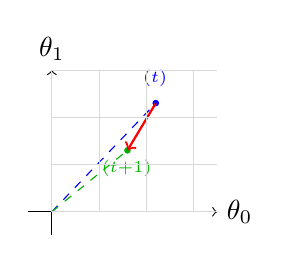
\begin{tikzpicture}[scale=0.6]
  % Axes
  \draw[->] (-0.5,0) -- (3.5,0) node[right] {$\theta_0$};
  \draw[->] (0,-0.5) -- (0,3) node[above] {$\theta_1$};
  
  % Points
  \coordinate (theta_t) at (2.2, 2.3);
  \coordinate (theta_t1_ols) at (1.6, 1.3);
  
  \fill[blue] (theta_t) circle (2pt);
  \fill[green!70!black] (theta_t1_ols) circle (2pt);
  
  % Vectors
  \draw[->, red, thick] (theta_t) -- (theta_t1_ols);
  
  % Norms
  \draw[dashed, blue] (0,0) -- (theta_t);
  \draw[dashed, green!70!black] (0,0) -- (theta_t1_ols);
  
  \node[blue, above] at (theta_t) {\small $\vtheta^{(t)}$};
  \node[green!70!black, below] at (theta_t1_ols) {\small $\vtheta^{(t+1)}$};
  
  % Grid
  \draw[gray!30, thin] (0,0) grid (3.5,3);
\end{tikzpicture}

\textbf{No shrinkage} \\
$\|\vtheta^{(t+1)}\|_2 = 1.98$
\end{center}

\column{0.48\textwidth}
\begin{center}
\textbf{Ridge Gradient Descent}
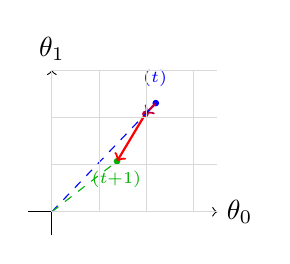
\begin{tikzpicture}[scale=0.6]
  % Axes
  \draw[->] (-0.5,0) -- (3.5,0) node[right] {$\theta_0$};
  \draw[->] (0,-0.5) -- (0,3) node[above] {$\theta_1$};
  
  % Points
  \coordinate (theta_t) at (2.2, 2.3);
  \coordinate (shrunk) at (1.98, 2.07);
  \coordinate (theta_t1_ridge) at (1.38, 1.07);
  
  \fill[blue] (theta_t) circle (2pt);
  \fill[purple] (shrunk) circle (2pt);
  \fill[green!70!black] (theta_t1_ridge) circle (2pt);
  
  % Vectors
  \draw[->, purple, thick] (theta_t) -- (shrunk);
  \draw[->, red, thick] (shrunk) -- (theta_t1_ridge);
  
  % Norms
  \draw[dashed, blue] (0,0) -- (theta_t);
  \draw[dashed, green!70!black] (0,0) -- (theta_t1_ridge);
  
  \node[blue, above] at (theta_t) {\small $\vtheta^{(t)}$};
  \node[green!70!black, below] at (theta_t1_ridge) {\small $\vtheta^{(t+1)}$};
  
  % Grid
  \draw[gray!30, thin] (0,0) grid (3.5,3);
\end{tikzpicture}

\textbf{With shrinkage} \\
$\|\vtheta^{(t+1)}\|_2 = 1.72$ \textcolor{red}{$<$ OLS}
\end{center}
\end{columns}

\begin{alertbox}{Ridge Effect}
Ridge regression systematically produces \textbf{smaller coefficient magnitudes} at every gradient descent step!
\end{alertbox}
\end{frame}

\begin{frame}{Summary: What We Learned}
\begin{keypointsbox}{Ridge Regression Key Points}
\begin{itemize}
\item \textbf{Problem}: Overfitting in linear regression with large coefficients
\item \textbf{Solution}: Add $L_2$ penalty $\lambda\|\vtheta\|_2^2$ to loss function
\item \textbf{Effect}: Shrinks coefficients, improves generalization
\item \textbf{Trade-off}: Higher bias, lower variance
\end{itemize}
\end{keypointsbox}
\end{frame}

\begin{frame}{Key Formula \& Next Steps}
\begin{theorembox}{Ridge Regression Solution}
$$\hat{\vtheta}_{\text{ridge}} = (\mX^T\mX + \lambda\mI)^{-1}\mX^T\vy$$
\end{theorembox}
\pause

\begin{alertbox}{Next Steps}
\begin{itemize}
\item Compare with Lasso regression ($L_1$ penalty)
\item Explore elastic net (combines $L_1$ and $L_2$)
\item Apply to real-world datasets
\end{itemize}
\end{alertbox}
\end{frame}


\end{document}
